\chapter{Anhang}

\begin{landscape}
	\section{Block-Design} \label{Appendix:BlockDesign}
	% Top level
	\begin{figure}[h] 
  		\centering
  		\textbf{Blockdesign: Top-Level}
  		\fbox{ 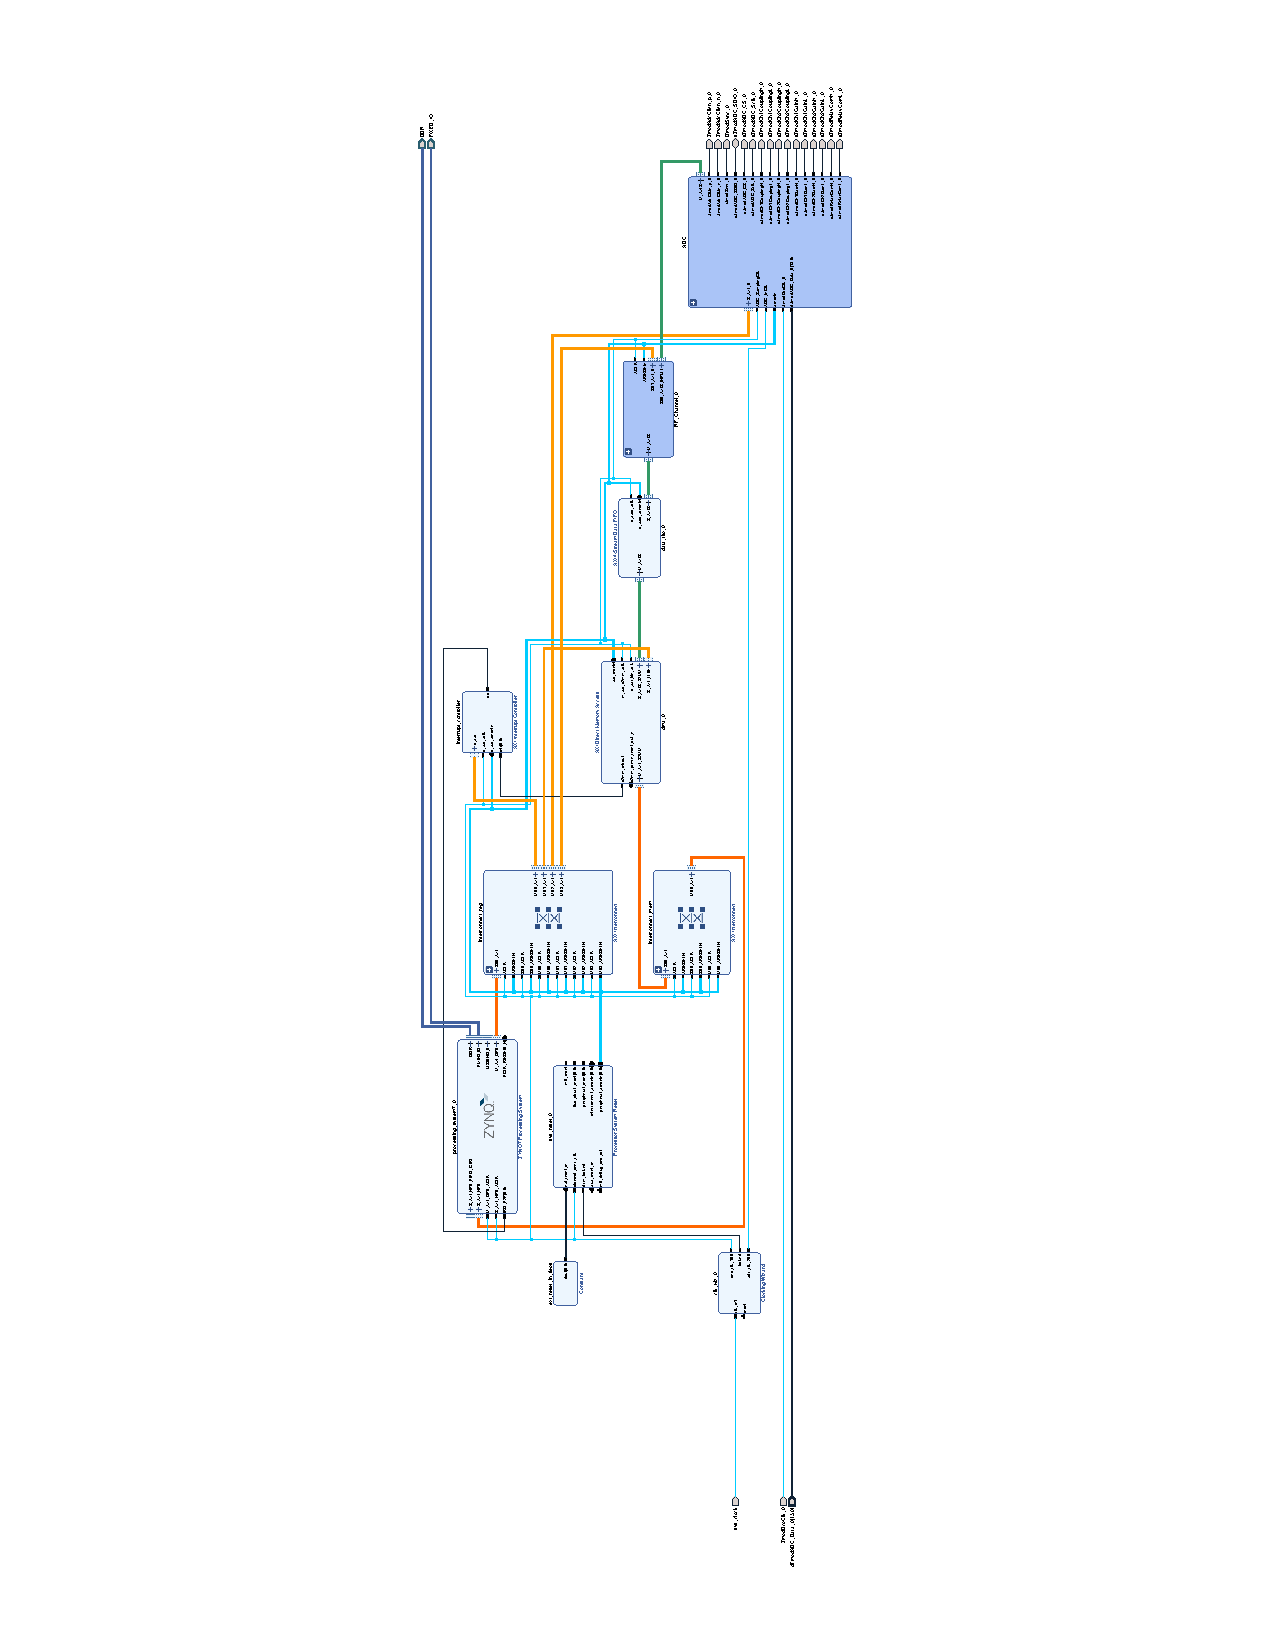
\includegraphics[angle=270,trim={7cm 1.5cm 7cm 1.5cm},clip,width=\linewidth]{export/design_1.pdf} }
  		\caption{Block-Design des Top-Level Moduls}
	\end{figure}
	
	% RF Channel 0
	\begin{figure}[h]
	  	\centering
		\textbf{Blockdesign: RF\_Channel\_0}
  		\fbox{ 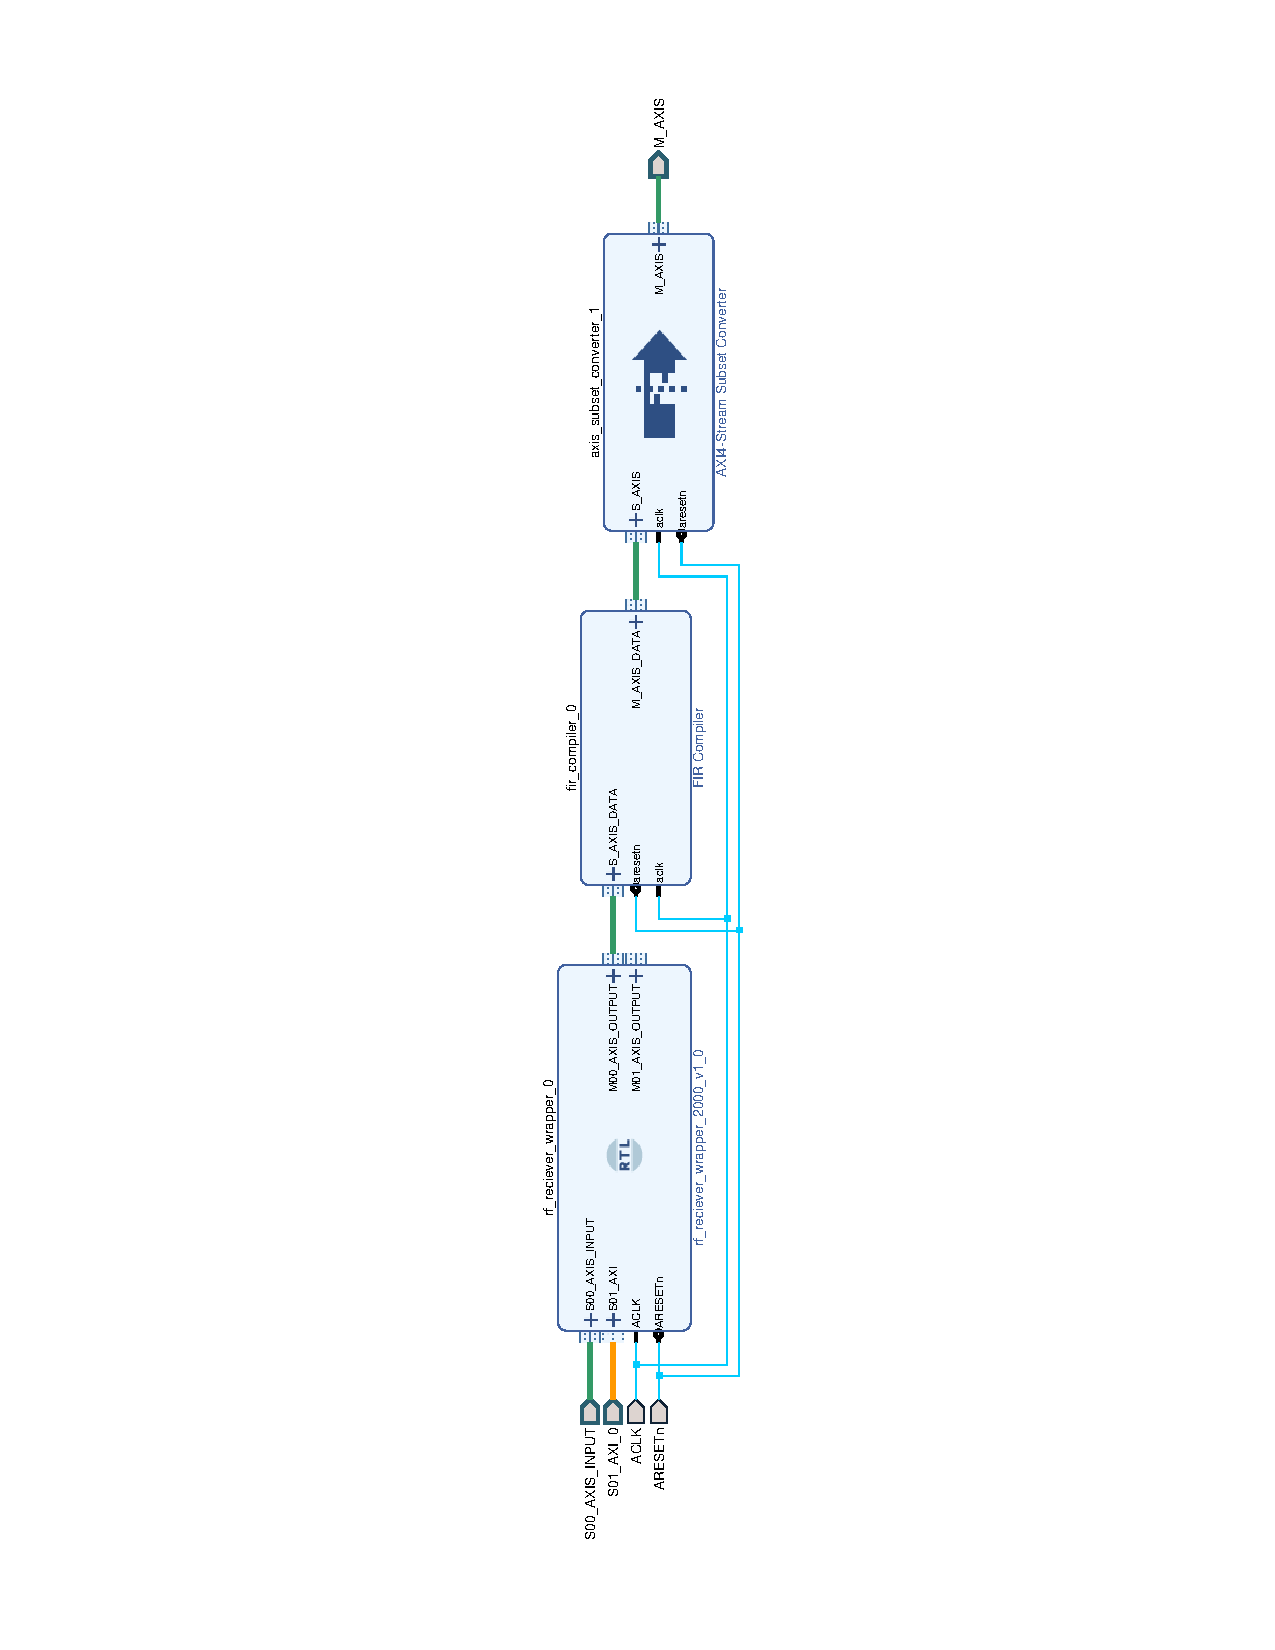
\includegraphics[angle=270,trim={7cm 1.5cm 7cm 1.5cm},clip,width=\linewidth]{export/RF_Channel_0.pdf} }
  		\caption{Block-Design des Sub-Blocks: RF Channel 0}
	\end{figure}
	
	% ADC
	\begin{figure}[h]
	  	\centering
		\textbf{Blockdesign: ADC}
  		\fbox{ 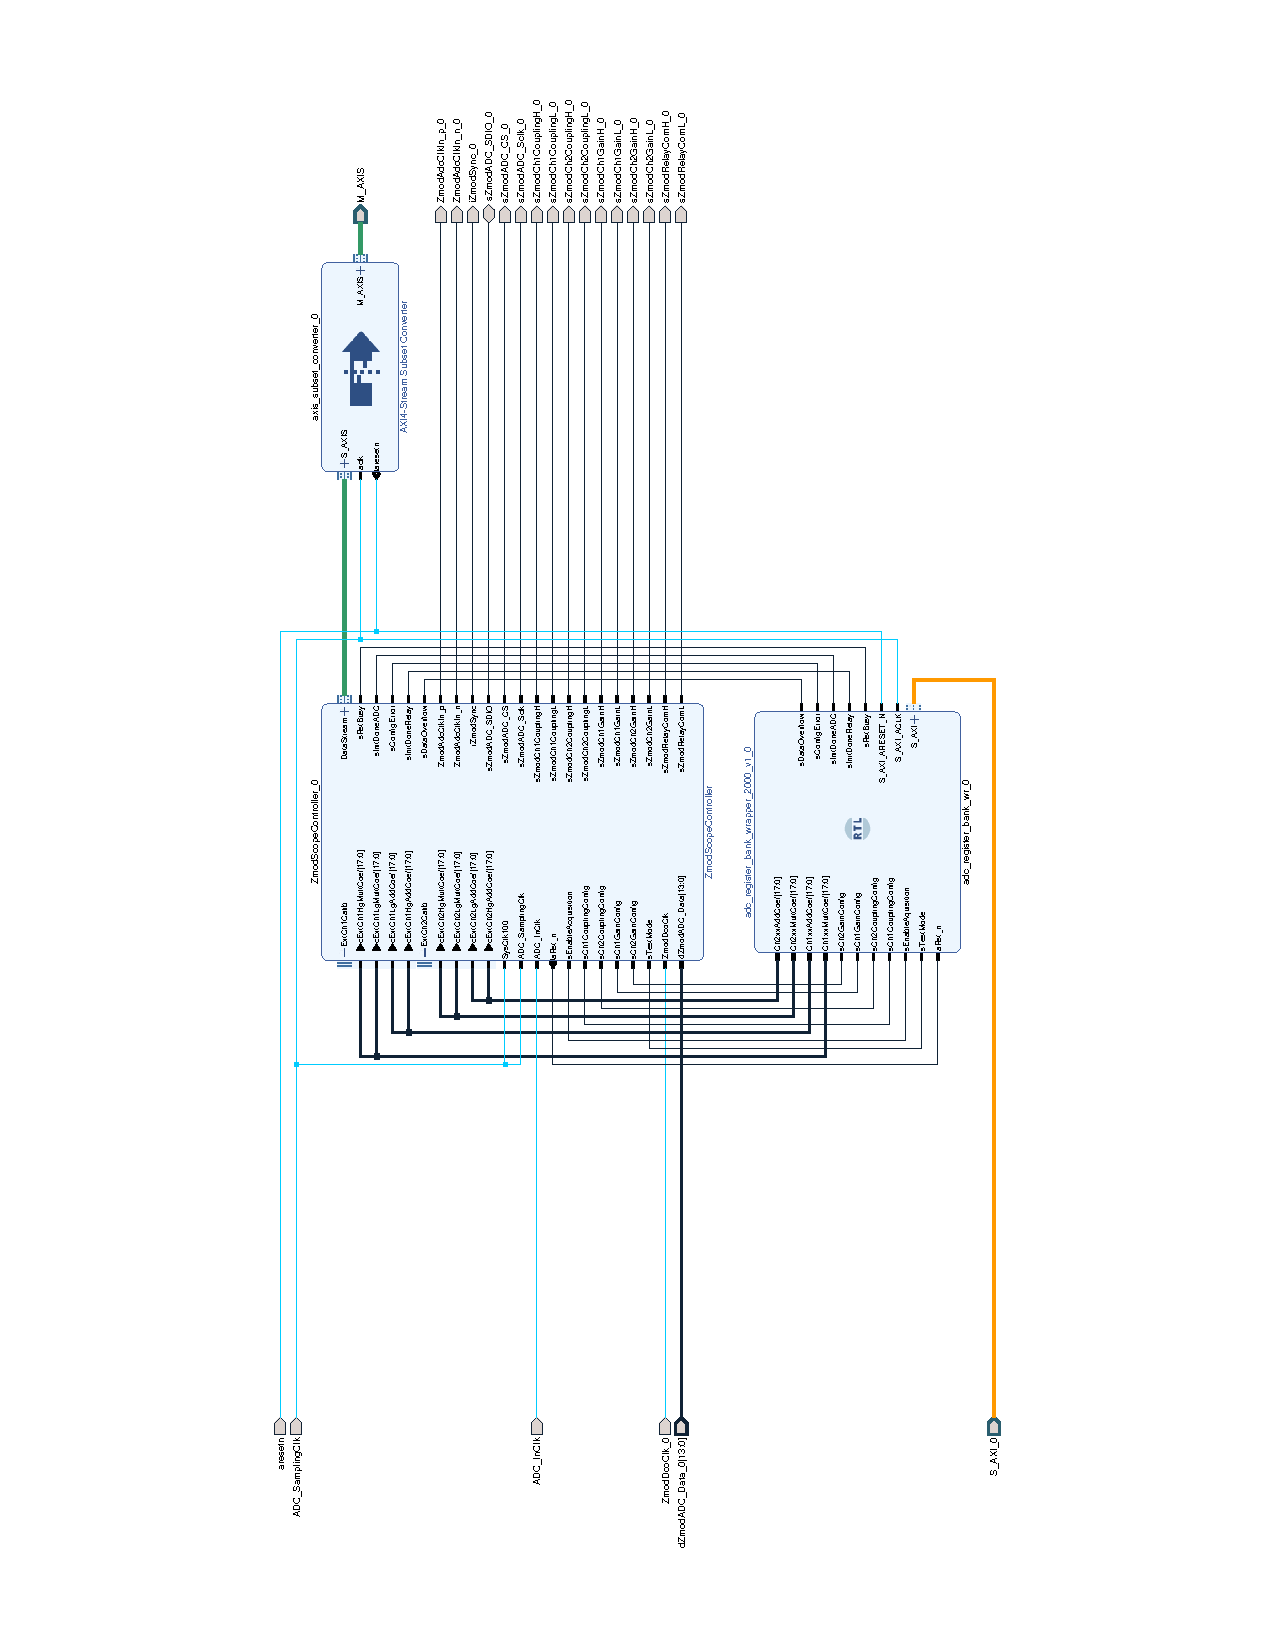
\includegraphics[angle=270,trim={4.5cm 1.5cm 4.5cm 1.5cm},clip,width=\linewidth]{export/ADC.pdf} }
  		\caption{Block-Design des Sub-Blocks: ADC}
	\end{figure}

\end{landscape}

\begin{figure}[ht]
	\section{Simulationsergebnis des RF-Recievers} \label{Appendix:Simulation}	
	  	\centering
	  	\includegraphics[trim={1.0cm 3cm 0.8cm 4.0cm},clip, width=\linewidth]{baseband}
  		\caption{Ergebnis der Simulation des RF-Recievers für: $f_c=\qty{20}{M\hertz}, \mathrm{SNR}=\qty{3}{dB}, A=\qty{-6}{dBFS}, \frac{\Delta f}{f_c} = \qty{-800}{ppm}$} 
  		\label{Abb:Result}
\end{figure}